\documentclass[8pt]{beamer}
\usetheme{Warsaw}
\usepackage{url}
\usepackage{multicol}
\usepackage[spanish]{babel}
\usepackage[utf8]{inputenc}
\usepackage{wrapfig}
\usepackage{booktabs}
 \usepackage{vwcol}  
%%
\title{Géneros, Alcohol y Tabaquismo: Somos tan diferentes?}
\author{Daniel Donalisio - Felix Rojo Lapalma}
\date{\today}

\begin{document}

\begin{frame}
\titlepage
\end{frame}

\section{Antes de Empezar}
%%%%%%%%%%%%%%%%%%%%%%%%%%%
\begin{frame}\frametitle{Disclaimer}
\begin{itemize}
\item El análisis fue realizado como anexo al Laboratorio 1 (bajo la seccion Anexo - Laoratorio 2). Los archivos fuente
pueden descargarse de \url{https://github.com/felixlapalma/diplodatos_2018}  
\item Hipótesis de uso: La presentación esta orientada a generar un conjunto de información que pudiera ser aprovechada por organismos
que realicen campa\~nas de concientizaci\'on relacionadas a los temas en estudio. Principalmente para contribuir a direccionar 
las acciones de un dado programa en forma y tiempo.
\item Si bien las presentaciones tienden a ser autocontenidas, algunas partes requieren del hilo conductor que gestiona el presentador de la misma.
\end{itemize}
Terminologia y notación: Usaremos en forma indistinta nombres en español o ingles para referirnos a género (gender), alcohol,tabaquismo (smoking) y cualquiera de las clases involucradas. \\
Hemos utilizado en forma indiscriminada tabaquismo (tabaco, etc) por \textit{smoking}. Esto puede no ser correcto coloquialmente en cuanto el dataset no especifica el tipo de elemento consumido. 
\end{frame}
%%%%%%%%%%%%%%%%%%%%%%%%

\section{Enfoque de problema y propuesta de acción}
\subsection{Que pretendemos entender y conocer?}
%%%%%%%%%%%%%%%%%%
\begin{frame}

\begin{block}{Análisis}
El presente abordaje esta enfocado en el análisis sobre igualdades y diferencias de género en cuanto a su
actitud respecto al alcohol y el tabaquismo.
\end{block}
\pause
\begin{block}{Que pretendemos conocer y entender?}
\begin{itemize}
\item La distribución de consumidores de tabaco por género.
\item La distribución de consumidores de alcohol por género.
\item La distribución etaria y por género de los que consumen alcohol y tabaco? Existe una edad en la que se da mas un hecho que otro?
\item ¿Como es la distribución en el caso de los consumidores sociales, son mas proclives a una edad? ¿Se diferencian por género?
\end{itemize}
\end{block}
\pause
\textbf{La lista anterior no pretende ser exhaustiva ni extensiva, sino simplemente plantear un \textit{road-map} que nos permita conocer 
un poco las igualdades y diferencias.}

\end{frame}

\subsection{Que acciones pretendemos tomar?}
%%%%%%%%%%%%%%%%%%%%%%%%%%%%%%%%%%%%%%%%%%%
\begin{frame}
\begin{alertblock}{Acciones}
A partir del análisis, ser capaces de generar información útil que pudiera ser aprovechada por organismos
que realicen campa\~nas de concientizacion relacionadas a los temas en estudio. Principalmente a direccionar 
esas campañas en forma y tiempo. Es decir, 
\pause
\begin{itemize}
\item \textbf{¿Tenemos que realizar un enfoque diferenciado respecto al género en el abordaje de temas como el alcoholismo y el tabaquismo?}
\end{itemize}
\end{alertblock}

\end{frame}

\section{Análisis - Consumo de Tabaco}
\subsection{Ditribuciones}
\begin{frame}\frametitle{Distribución}
\setlength{\columnsep}{80pt} 
\begin{multicols}{2}
 \begin{minipage}[t]{.6\textwidth}
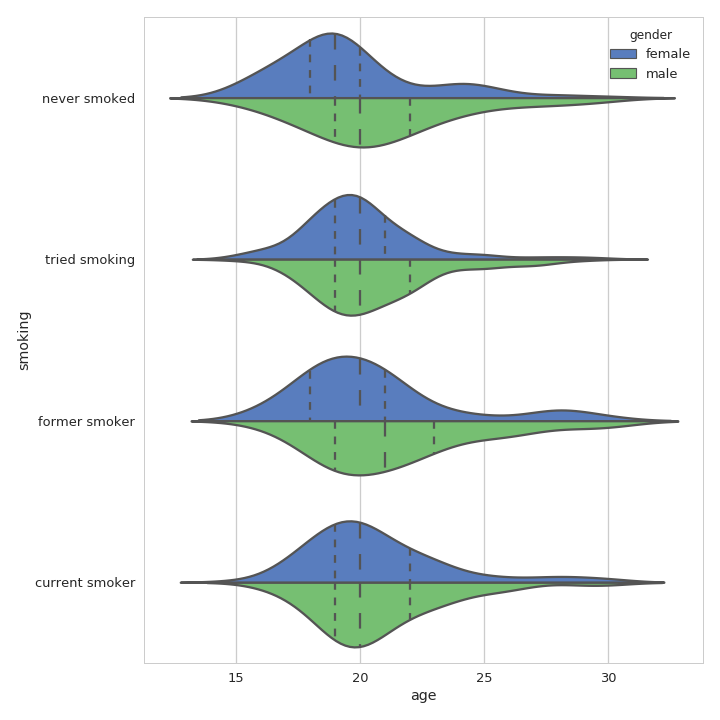
\includegraphics[scale=0.25]{smoking_dist}
\end{minipage}

\begin{minipage}[t]{.4\textwidth}
\tiny{
\begin{block}{never smoked}
Existe un diferencia entre géneros, no en forma funcional, sino en su localización (observar los quartiles en la misma figura). Esto podria indicar  que es necesario un tratamiento diferenciado en cuanto al género.
\end{block}
\pause
\begin{block}{tried smoking}
Muestra una paridad entre géneros respecto a su distribucion (aunque el género masculino tiende a tener mas intentos a mayor edad).
\end{block}
\pause
\begin{block}{former smoker}
Similar a \textit{never smoked}, la forma funcional del nucleo de la distribución parece estar desplazado pero no su forma.
\end{block}
\begin{block}{current smoker}
No se observan diferencias evidentes para las/los actuales fumadores.
\end{block}
}
\end{minipage}
\end{multicols}
\end{frame}


\subsection{Supervivencia de un Comportamiento}
%%%%%%%%%%%%%%%%%%%%%%%%%%%%%%%%%%%%%%%%%%%%%%%%%%%%%%%%%%%%%%%%%%%%%%
\begin{frame}
A los comentarios anteriores les podemos dar soporte extra considerando, dado un evento, su probabilidad de supervivencia, la cual 
no es mas que $\Phi(t)=1-FDA(t)$  (para FDA función de densidad acumulada).

\setlength{\columnsep}{80pt} 
\begin{multicols}{2}
\begin{minipage}[t]{0.6\textwidth}
 \begin{figure}
 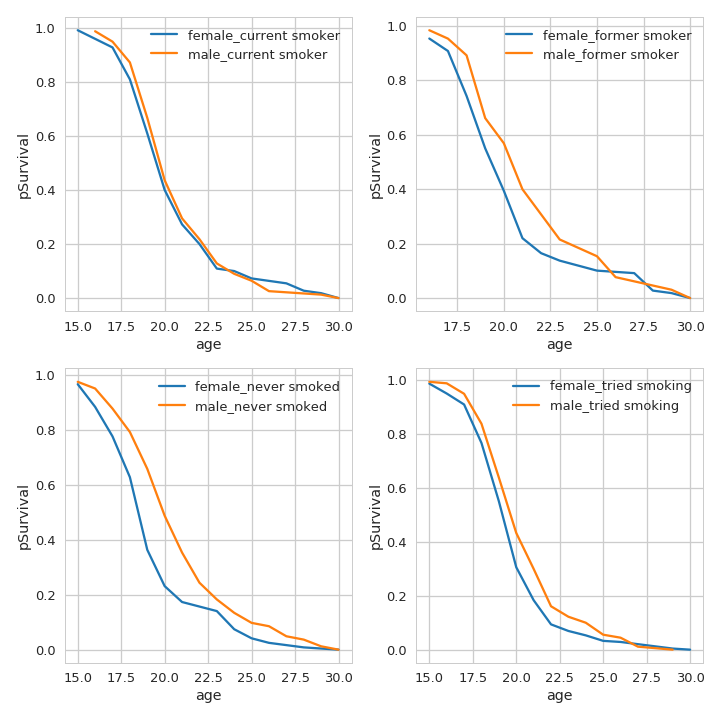
\includegraphics[scale=0.25]{smoking_survival}
 \end{figure}
  \end{minipage}
\begin{minipage}[t]{0.4\textwidth}
\begin{block}{Supervivencia de un Comportamiento}
Las probabilidades de supervivencia graficadas vemos que hacen plausibles las suposiciones en cuanto a diferencias o similitudes 
(en las distribuciones). En virtud de estas podriamos generar ciertos indicativos, en este caso que, el enfoque respecto a los 
grupos de consumo deberia empezar en forma mas temprana para el género femenino.
\end{block}
\end{minipage}
\end{multicols}
\end{frame}

\subsection{Outliers}
%%%%%%%%%%%%%%%%%%%%%%%%%%%%%%%%%%%%%%%%%%%%%%%%%%%%%%%%%%%%%%%%%%%%
%%%% FALTA
\begin{frame}\frametitle{Outliers}
En proceso ...
% \begin{figure}
% 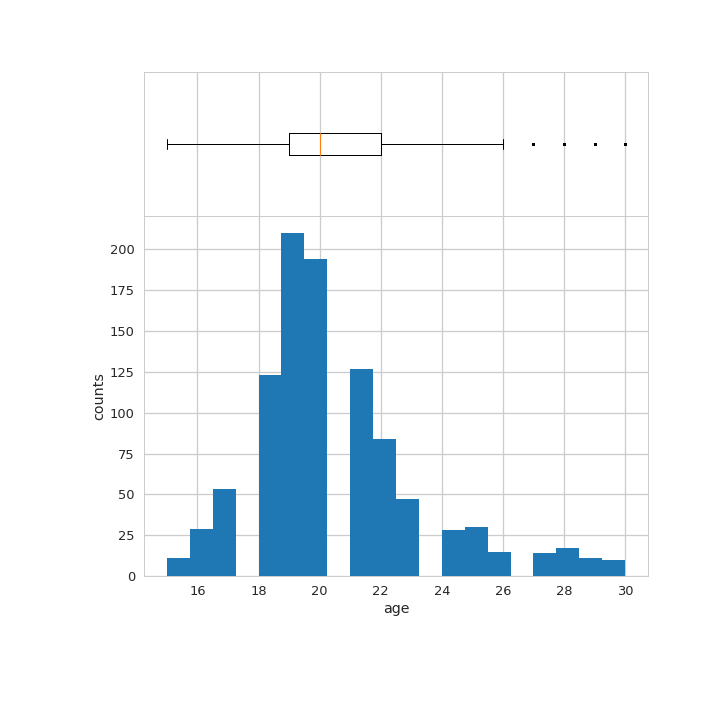
\includegraphics[scale=0.1]{age_hist}
% \end{figure}
% \begin{figure}
% 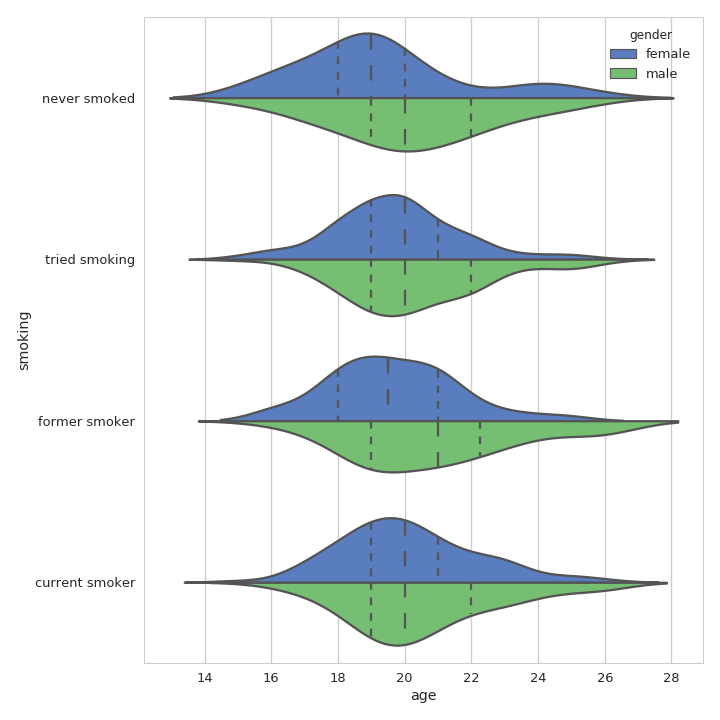
\includegraphics[scale=0.1]{smoking_dist_woo}
% \end{figure}
\end{frame}

\subsection{Clases y $\chi^2$ }
%%%%%%%%%%%%%%%%%%%%%%%%%%%%%%%%%%%%%%%%%%%%%%%%%%%%%%%%%%%%%%%%%%%%%
\begin{frame}
Veamos (ya sin la distribución de edad) como se distribuye por género el tabaquismo, 
\tiny{
\begin{table}
\begin{tabular}{lrrrr}
\toprule
{} &  current smoker &  former smoker &  never smoked &  tried smoking \\
\midrule
female &              70 &             70 &            86 &            176 \\
male   &              48 &             45 &            59 &            120 \\
\bottomrule
\end{tabular}
\end{table}
} 
\small{Un primer vistazo a la tabla no arroja grandes diferencias por clase. Y se observa en forma similar para las cuentas normalizadas,}
\tiny{
\begin{table}
\begin{tabular}{lrrrr}
\toprule
{} &  current smoker &  former smoker &  never smoked &  tried smoking \\
\midrule
female &        0.174129 &       0.174129 &      0.213930 &       0.437811 \\
male   &        0.176471 &       0.165441 &      0.216912 &       0.441176 \\
\bottomrule
\end{tabular}
\end{table} 
}
\begin{multicols}{2}
  \begin{figure}
 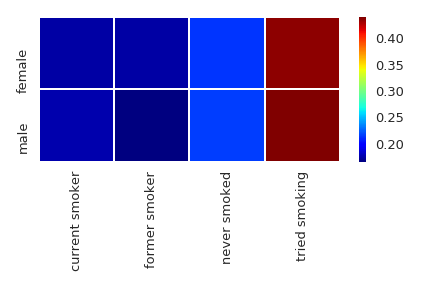
\includegraphics[scale=0.3]{smoking_heatmap}
 \end{figure}
 \columnbreak
\small{En este formato vemos que son similares las proporciones por clase (tanto numericamente como graficamente). Veamos que nos puede decir el test $\chi^2$.} 
\end{multicols}
\end{frame}


\begin{frame}
Es decir buscamos responder si las diferencias observadas en los grupos son relacionadas al azar o tienen una correlacion o de otra forma \textit{si la actitud respecto al tabaquismo se distribuye de la misma manera independiente del género}. 

\begin{table}
\begin{tabular}{lccc}
\toprule
{} &  $\chi^2$ &  $p-value$ &  $dof$  \\
\midrule
valor &        0.08 &       0.99 &      3  \\
\bottomrule
\end{tabular}
\end{table} 
\pause
\begin{exampleblock}{Recordemos...}
Cuanto mayor sea el valor de $\chi^2$ , menos verosímil es que la hipótesis nula (que asume la igualdad entre ambas distribuciones) sea correcta. De la misma forma, cuanto más se aproxima a cero el valor de $\chi^2$, más ajustadas están ambas distribuciones. 
\end{exampleblock}
\pause
\begin{block}{}
En función de los resultados podemos decir que las distribuciones parecen tener un origen común (es decir la actitud respecto al tabaquismo parece tener un mismo comportamiento entre géneros). La significancia estadística la vemos en terminos del $p$-valor. El valor $p$ nos muestra la probabilidad de haber obtenido el resultado que hemos obtenido si suponemos que la hipótesis nula es cierta. En nuestro caso $p>0.99$ con lo cual \textbf{NO} podemos rechazar la hipotesis de que los datos provengan de una misma distribución y las diferencias solo sean debidas al azar.
\end{block}
\end{frame}


\subsection{Resumen - Consumo de tabaco}
%%%%%%%%%%%%%%%%%%%%
\begin{frame}
En relación al procesamiento de los datos, podemos realizar un par de observaciones,
\pause
\begin{block}{Sobre las distribuciones, y comportamientos condicionados por edad}
El análisis realizado indica que el comportamiento en relación a la actitud a ciertas fases del tabaquismo, parece diferenciar
los generos. Particularmente la fases de \textit{nunca consumió (never smoked)} e \textit{intentó consumir (tried smoking)} parecen
exigir un tratamiento por género.  
\end{block}

\pause
\begin{block}{Sobre el comportamiento en general}
El test $\chi^2$ parece indicar un origen comun en el comportamiento general o actitud hacia el consumo de tabaco. 
\end{block} 

\pause
\begin{alertblock}{Acciones}
Las comentarios previos indican que \textbf{No} somos tan diferentes - por género - en cuanto a nuestra actitud hacia el tabaco. Es decir
un enfoque unificado seria de utilidad para ambos géneros (en consideración).  Al margen que deberian ajustarse ciertos tiempos de aplicación de estos enfoques.
\end{alertblock} 

\end{frame}



\section{Análisis - Consumo de Alcohol}
%%%%%%%%%%%%%%%%%%%%%%%%%%%%%%%%%%%%%%%%%%%%%%%%%%%%%%%%%%%%%%%%%%%%%%%%%%%%%%%%%
\subsection{Distribuciones}
%%%%%%%%%%%%%%%%%%%%%%%%%%%%%%%%%%%%%%%%%%%%%%%%%%%%%%%%%%%%%%%%%%%%%%%%%%%%%%%%%
\begin{frame}\frametitle{Distribución}

\setlength{\columnsep}{80pt} 
\begin{multicols}{2}
\begin{minipage}[t]{.6\textwidth}
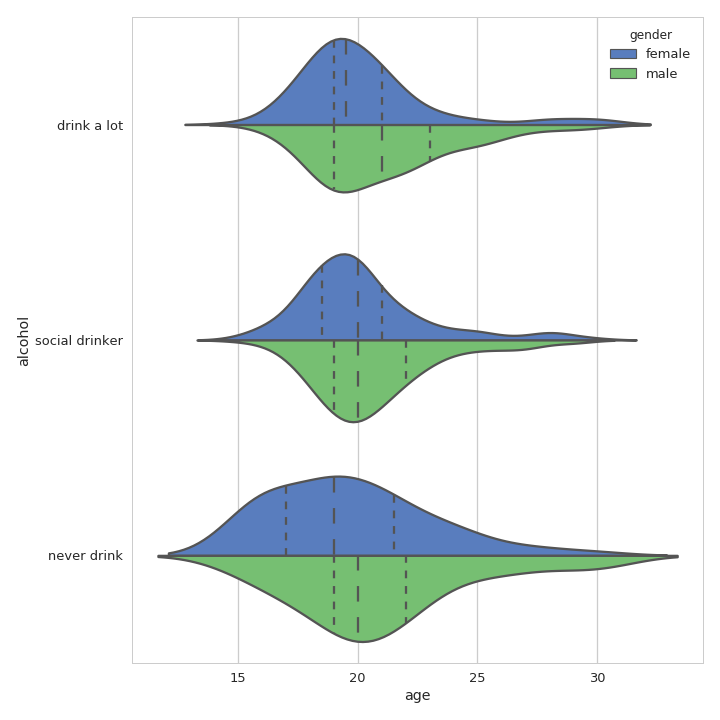
\includegraphics[scale=0.25]{alcohol_dist}
\end{minipage}
%
\begin{minipage}[t]{.4\textwidth}
\tiny{
\begin{block}{never drink}
Parece existir una diferencia entre géneros, no en forma funcional para la distribución 
sino en su localizacion (observar quartiles en la misma figura).
\end{block}
\pause
\begin{block}{social drinker}
Muestra una paridad entre géneros respecto a su distribución (aunque el género masculino tiende a tener mas intentos a mayor edad).
\end{block}
\pause
\begin{block}{drink a lot}
Muestra una paridad entre géneros (aunque la mediana para el género masculino se encuentra en una edad mayor que en el caso femenino).
\end{block}
}
\end{minipage}
\end{multicols}


\end{frame}

\subsection{Supervivencia de un comportamiento}
%%%%%%%%%%%%%%%%%%%%%%%%%%%%%%%%%%%%%%%%%%%%%%%%%%%%%%%%%%%%%%%%%%%%%%
\begin{frame}
A los comentarios anteriores les podemos dar soporte extra considerando, dado un evento, su probabilidad de supervivencia, la cual 
no es mas que $\Phi(t)=1-FDA(t)$  (para FDA función de densidad acumulada).

\setlength{\columnsep}{60pt} 
\begin{multicols}{2} 
\begin{minipage}[t]{.6\textwidth}
\begin{figure}
 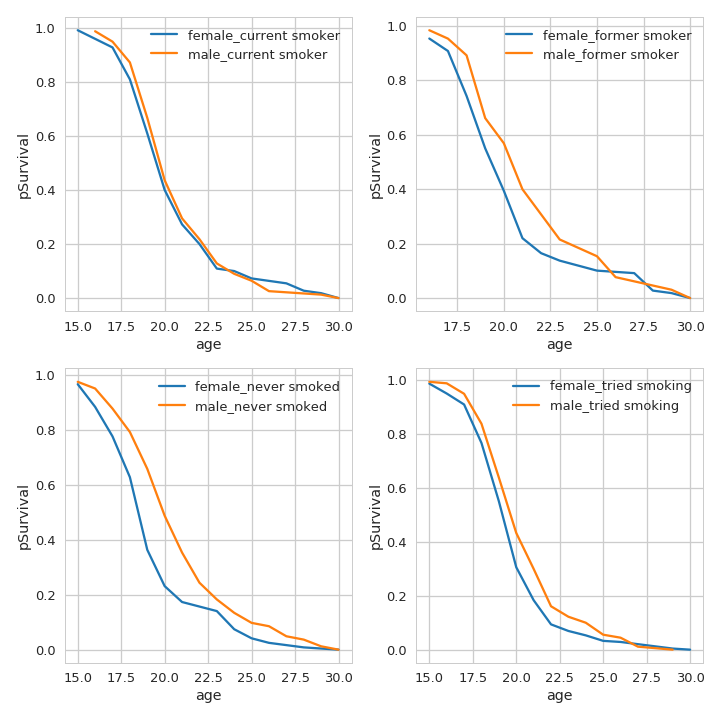
\includegraphics[scale=0.25]{smoking_survival}
 \end{figure}
\end{minipage}
\begin{minipage}[t]{.4\textwidth}
\pause
\centering
\small{
\begin{block}{Supervivencia de un comportamiento}
Las probabilidades de supervivencia graficadas vemos que dan soporte a las suposiciones en cuanto a diferencias o similitudes (en las distribuciones). En virtud de estas podriamos generar ciertos indicativos, en este caso, estan indicando que se deberia abordar en forma diferenciada el consumo excesivo de alcohol en el género masculino.
\end{block}
}
\end{minipage} 
\end{multicols}
\end{frame}

\subsection{Outliers}
\begin{frame}\frametitle{Outliers}
\begin{multicols}{2} 
 \begin{figure}
 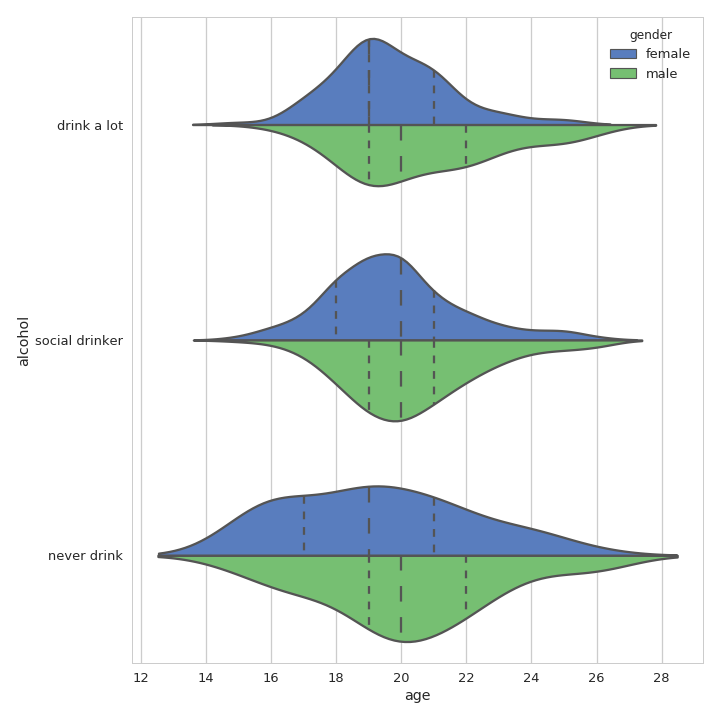
\includegraphics[scale=0.2]{alcohol_dist_woo}
 \end{figure}
 \columnbreak
 \begin{figure}
 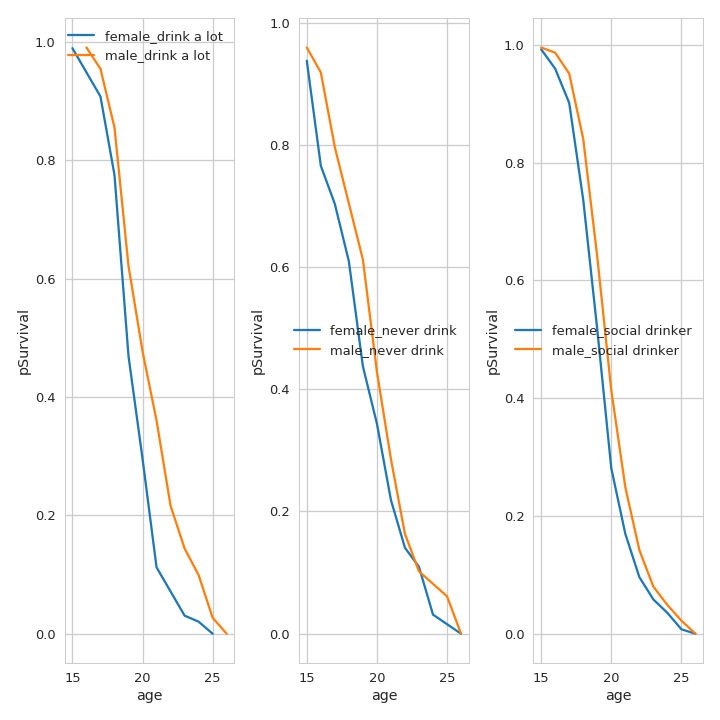
\includegraphics[scale=0.2]{alcohol_survival_woo}
 \end{figure}
 \end{multicols}
 \small{La remoción de outliers no parece alterar en forma significativa ninguna de las distribuciones representadas. Esto con la salvedad que en el caso de grandes consumidores se marca mas definidamente la existencia de cierta asimetría en la permanencia de consumidores a edades mayores en el género masculino sobre el género femenino.} 
\end{frame}

\subsection{Clases y $\chi^2$ }
%%%%%%%%%%%%%%%%%%%%%%%%%%%%%%%%%%%%%%%%%%%%%%%%%%%%%%%%%
\begin{frame}
Veamos (sin condicionar por edades) como se distribuye por género el consumo de alcohol,
\tiny{
\begin{table}
\begin{tabular}{lccc}
\toprule
{} &  drink a lot &  never drink &  social drinker \\
\midrule
female &           74 &           40 &             288 \\
male   &           79 &           33 &             160 \\
\bottomrule
\end{tabular}
\end{table} 
}
\small{Un primer vistazo a la tabla arroja cierta asimetría en una de las clasificaciones. Y si observamos en cuentas normalizadas,}
\tiny{
\begin{table}
\begin{tabular}{lccc}
\toprule
{} &  drink a lot &  never drink &  social drinker \\
\midrule
female &     0.184080 &     0.099502 &        0.716418 \\
male   &     0.290441 &     0.121324 &        0.588235 \\
\bottomrule
\end{tabular}
\end{table} 
}
%
\begin{multicols}{2}
  \begin{figure}
 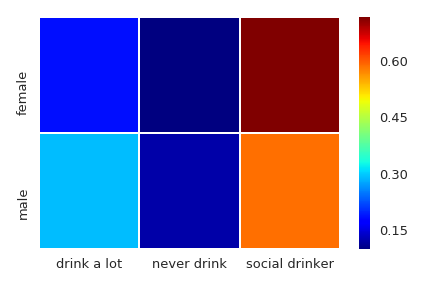
\includegraphics[scale=0.3]{alcohol_heatmap}
 \end{figure}
 \small{En este formato vemos que las proporciones por clase (tanto numericamente como graficamente) tienden a diferenciarse. Veamos que nos puede decir el test $\chi^2$ de Person respecto a esto.}
 \end{multicols}
\end{frame}

\begin{frame}\frametitle{$\chi^2$}
%
Es decir buscamos responder si las diferencias observadas en los grupos son relacionadas al azar o tienen una correlación o de otra forma \textit{si la actitud respecto al alcohol se distribuye de la misma manera independiente del género}. 
%
\begin{table}
\begin{tabular}{lrrr}
\toprule
{} &  $\chi^2$ &  $p-value$ &  $dof$  \\
\midrule
valor &        12.8 &       0.0016 &      2  \\
\bottomrule
\end{tabular}
\end{table} 
\pause
\begin{block}{}
En funcion de lo obtenido podemos decir que las distribuciones parecen tener un origen distinto (es decir la actitud respecto al consumo de alcohol parece tener un comportamiento diferente entre géneros). La significancia estadistica la vemos en terminos del $p$-valor. El valor $p$ nos muestra la probabilidad de haber obtenido el resultado que hemos obtenido si suponemos que la hipótesis nula es cierta.  En nuestro caso $p<0.001 (p_{\%}<0.16\%)$ con lo cual \textbf{SI} podemos rechazar la hipótesis de que los datos provengan de una misma distribución.
\end{block}
\end{frame}



\subsection{Resumen - Consumo de alcohol}
%%%%%%%%%%%%%%%%%%%%
\begin{frame}[shrink=10]
En relación al procesamiento de los datos, podemos realizar un par de observaciones,
\pause
\begin{block}{Sobre las distribuciones, y comportamientos condicionados por edad}
El análisis realizado indica que el comportamiento en relación a la actitud a ciertas fases del alcoholismo, parece diferenciar
los generos. Particularmente dos de las tres fases indican un comportamiento diferenciado en cuanto a lo temporal. Por caso, el genero
femenino parece tener una transición mas acelerada en el caso de alto consumo, lo cual en si mismo parece mejor, puesto que lo abandona en forma
mas temprana, pero seria necesario entender esta situación. En el lado opuesto, el género masculino en terminos de edad alcanza mas tarde esta condicion y su permanencia es mas extendida, con lo que exigiria un analisis del porque de su permanencia para orientar acciones en este punto.   
\end{block}

\pause
\begin{block}{Sobre el comportamiento en general}
El test $\chi^2$ parece indicar un origen diferenciado en el comportamiento general o actitud hacia el consumo de alcohol. 
\end{block} 

\pause
\begin{alertblock}{Acciones}
Las comentarios previos indican que \textbf{Si} parecemos mantener diferencias - por género - en cuanto a nuestra actitud hacia el alcohol. Es decir
un enfoque diferenciado seria de utilidad para ambos géneros (en consideración). Asimismo en este enfoque diferenciado deberian ajustarse ciertos tiempos de aplicacion (consistentes para cada genero).
\end{alertblock} 
\end{frame}





\section{Comentarios Finales}
%%%%%%%%%%%%%%%%%%%%%%%%%%%%%%%%%%%%%%%%%%%%
\begin{frame}
En esta sección recolectamos simplemente el conjunto de acciones y las dejamos en consideración,
\pause
\begin{alertblock}{Acciones}
Las comentarios previos indican que \textbf{No} somos tan diferentes - por género - en cuanto a nuestra actitud hacia el tabaco. Es decir
un enfoque unificado seria de utilidad para ambos géneros (en consideración).  Al margen que deberian ajustarse ciertos tiempos de aplicacion de estos enfoques.
\end{alertblock}  

\pause
\begin{alertblock}{Acciones}
Las comentarios previos indican que \textbf{Si} parecemos mantener diferencias - por género - en cuanto a nuestra actitud hacia el alcohol. Es decir
un enfoque diferenciado seria de utilidad para ambos géneros (en consideración). Asimismo en este enfoque diferenciado deberian ajustarse ciertos tiempos de aplicacion (consistentes para cada género).
\end{alertblock} 

\end{frame}

%%
\begin{frame}
\begin{center}
\huge{Preguntas?}\\ [1cm]
\Large{Gracias!}
\end{center}
\end{frame}


\end{document}
\grid
